\documentclass[12pt]{standalone}
\usepackage{tikz, etoolbox}
\usetikzlibrary{arrows.meta, positioning, shapes, shapes.geometric, calc}

% Sanserif font:
\renewcommand{\familydefault}{\sfdefault}

\newcommand{\entity}[3][]{
  \node(#2)[
    entity,
    #1
  ] {
    \nodepart[font=\bfseries]{one} #2
    \nodepart{two} #3
  };
}

\tikzset{
  entity/.style = {
    draw,
    align=left,
    rectangle split,
    rectangle split parts=2,
    rectangle split ignore empty parts,
    rectangle split part align={center, left},
    minimum width=3cm,
  },
  parallellogram/.style = {
    draw,
    trapezium,
    trapezium left angle=75,
    trapezium right angle=105,
  },
  onArrow/.style = {
    fill=white,
    align=center,
  },
  has/.style = {
    -{Latex[length=3mm]},
  },
  inherits/.style = {
    -{Latex[open, length=3mm]},
  },
  bigArrow/.style = {
    -{Latex[length=5mm]},
    line width=1mm,
    font=\bfseries,
  },
  node distance=2cm and 1cm,
}

% Attempt to get a little border padding
% \usepackage[
%     left=0.20in,
%     right=0.20in,
%     top=0.20in,
%     bottom=0.20in,
% ]{geometry}


\begin{document}

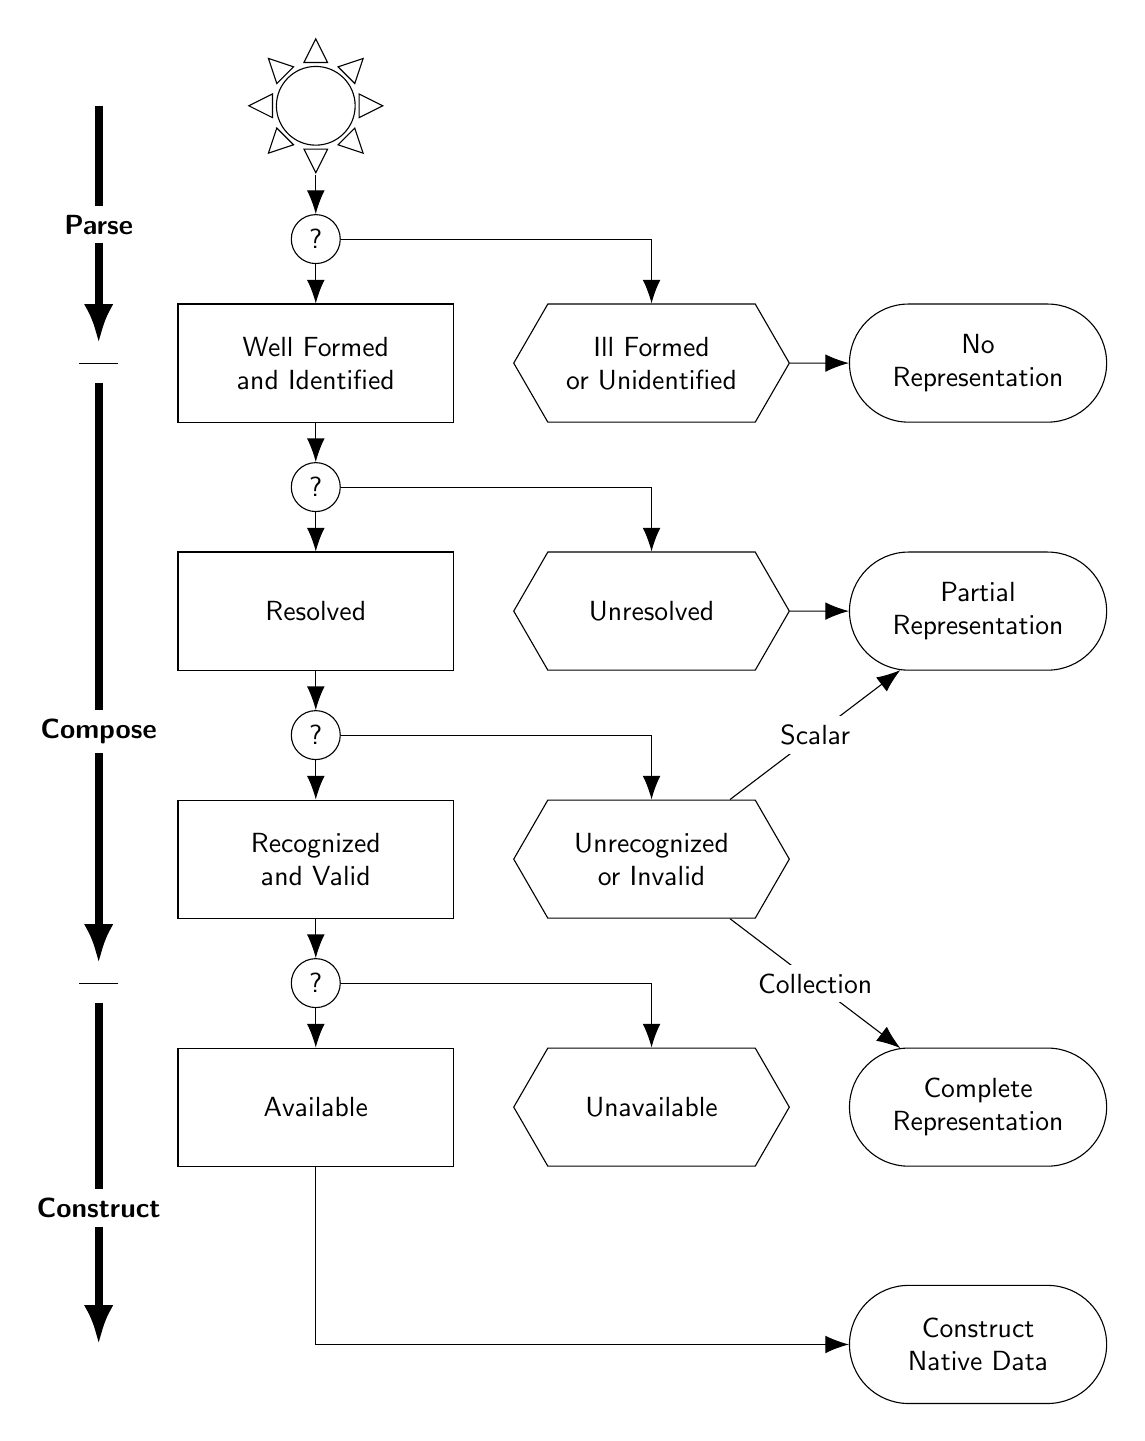
\begin{tikzpicture}[
  rect/.style = {
    draw,
    rectangle,
    align=center,
    minimum width=3.5cm,
    minimum height=1.5cm,
  },
  hex/.style = {
    rect,
    signal,
    signal to={west and east},
    signal pointer angle=120,
  },
  rounded/.style = {
    rect,
    rounded rectangle,
  },
  decision/.style = {
    draw,
    circle,
    node contents=?,
  },
  goes/.style = {
    -{Latex[length=3mm]},
  },
  bigArrow/.style = {
    -{Latex[length=5mm]},
    line width=1mm,
  },
]

\matrix[
  row sep=.5cm,
  column sep=.75cm,
] {

  \node[circle, minimum size=1.75cm](Start) {};
  \draw node[draw, circle, minimum size=1cm] at (Start) {};
  \foreach \angle in { 45, 90,..., 360 }{
    \draw [rotate around={\angle:(Start)}]
      (.55,0) -- +(0,-.15) -- +(.3,0) -- +(0,.15) -- cycle;
  }; \\

  \node(Q1)[decision]; \\
  \node(Well)[rect] {Well Formed\\and Identified}; &
  \node(Ill)[hex] {Ill Formed\\or Unidentified}; &
  \node(No)[rounded] {No\\Representation}; \\

  \node(Q2)[decision]; \\
  \node(Resolved)[rect] {Resolved}; &
  \node(Unresolved)[hex] {Unresolved}; &
  \node(Partial)[rounded] {Partial\\Representation}; \\

  \node(Q3)[decision]; \\
  \node(Recognized)[rect] {Recognized\\and Valid}; &
  \node(Unrecognized)[hex] {Unrecognized\\or Invalid};\\

  \node(Q4)[decision]; \\
  \node(Available)[rect] {Available}; &
  \node(Unavailable)[hex] {Unavailable}; &
  \node(Complete)[rounded] {Complete\\Representation}; \\[1cm]

  & & \node(Native)[rounded] {Construct\\Native Data}; \\
};

\draw[goes] (Start) -- (Q1);
\draw[goes] (Q1) -- (Well);
\draw[goes] (Q1) -| (Ill);
\draw[goes] (Ill) -- (No);

\draw[goes] (Well) -- (Q2);
\draw[goes] (Q2) -- (Resolved);
\draw[goes] (Q2) -| (Unresolved);
\draw[goes] (Unresolved) -- (Partial);

\draw[goes] (Resolved) -- (Q3);
\draw[goes] (Q3) -- (Recognized);
\draw[goes] (Q3) -| (Unrecognized);
\draw[goes] (Unrecognized) -- node[onArrow] {Scalar} (Partial);
\draw[goes] (Unrecognized) -- node[onArrow] {Collection} (Complete);

\draw[goes] (Recognized) -- (Q4);
\draw[goes] (Q4) -- (Available);
\draw[goes] (Q4) -| (Unavailable);

\draw[goes] (Available) |- (Native);

\draw let
  \p1 = (Start),
  \p2 = ($(Well.west)+(-1,0)$),
  \p3 = (Q4),
  \p4 = (Native),
in
  coordinate(C1) at (\x2,\y1)
  coordinate(C2) at (\x2,\y2)
  coordinate(C3) at (\x2,\y3)
  coordinate(C4) at (\x2,\y4)
;

\draw[bigArrow] (C1) -- node[onArrow, font=\bfseries] {Parse} ($(C2)+(0,0.25)$);
\draw[bigArrow] ($(C2)-(0,.25)$) -- node[onArrow, pos=.6, font=\bfseries] {Compose} ($(C3)+(0,0.25)$);
\draw[bigArrow] ($(C3)-(0,.25)$) -- node[onArrow, pos=.6, font=\bfseries] {Construct} (C4);

\draw ($(C2)-(.25,0)$) -- ($(C2)+(.25,0)$);
\draw ($(C3)-(.25,0)$) -- ($(C3)+(.25,0)$);

\end{tikzpicture}

\end{document}
